\section{Methodik}

\subsection{Datenbeschaffung und -aufbereitung}

\subsection{Contraction Hierarchies}
\subsubsection{Überblick}
Straßennetzwerke weisen eine sehr hierarchische Struktur auf. Es gibt "`wichtigere"' Straßen wie \zB Autobahnen
und "`unwichtigere"' Straßen wie \zB Straßen in Wohnsiedlungen (siehe
Abbildung~\ref{fig:road_hierarchy}). Um von einem entfernten Ort zu einem anderen zu gelangen, ist
es daher nur sinvoll, sich über Straßen mit zunehmender Wichtigkeit zu bewegen. Bei einer Suche könnte die
Information des Straßentyps und der damit verbundenen Wichtigkeit als Heuristik verwendet werden, um
bestimmte Kanten, die auf weniger wichtige Straßen führen,  zu ignorieren und damit die Suche zu
beschleunigen. Das Problem hierbei ist allerding, dass mit dieser Methode keine Garantie besteht,
dass der gefundene Weg auch wirklich der \emph{exakt} kürzeste Weg ist.
\begin{figure}[h]
    \centering
    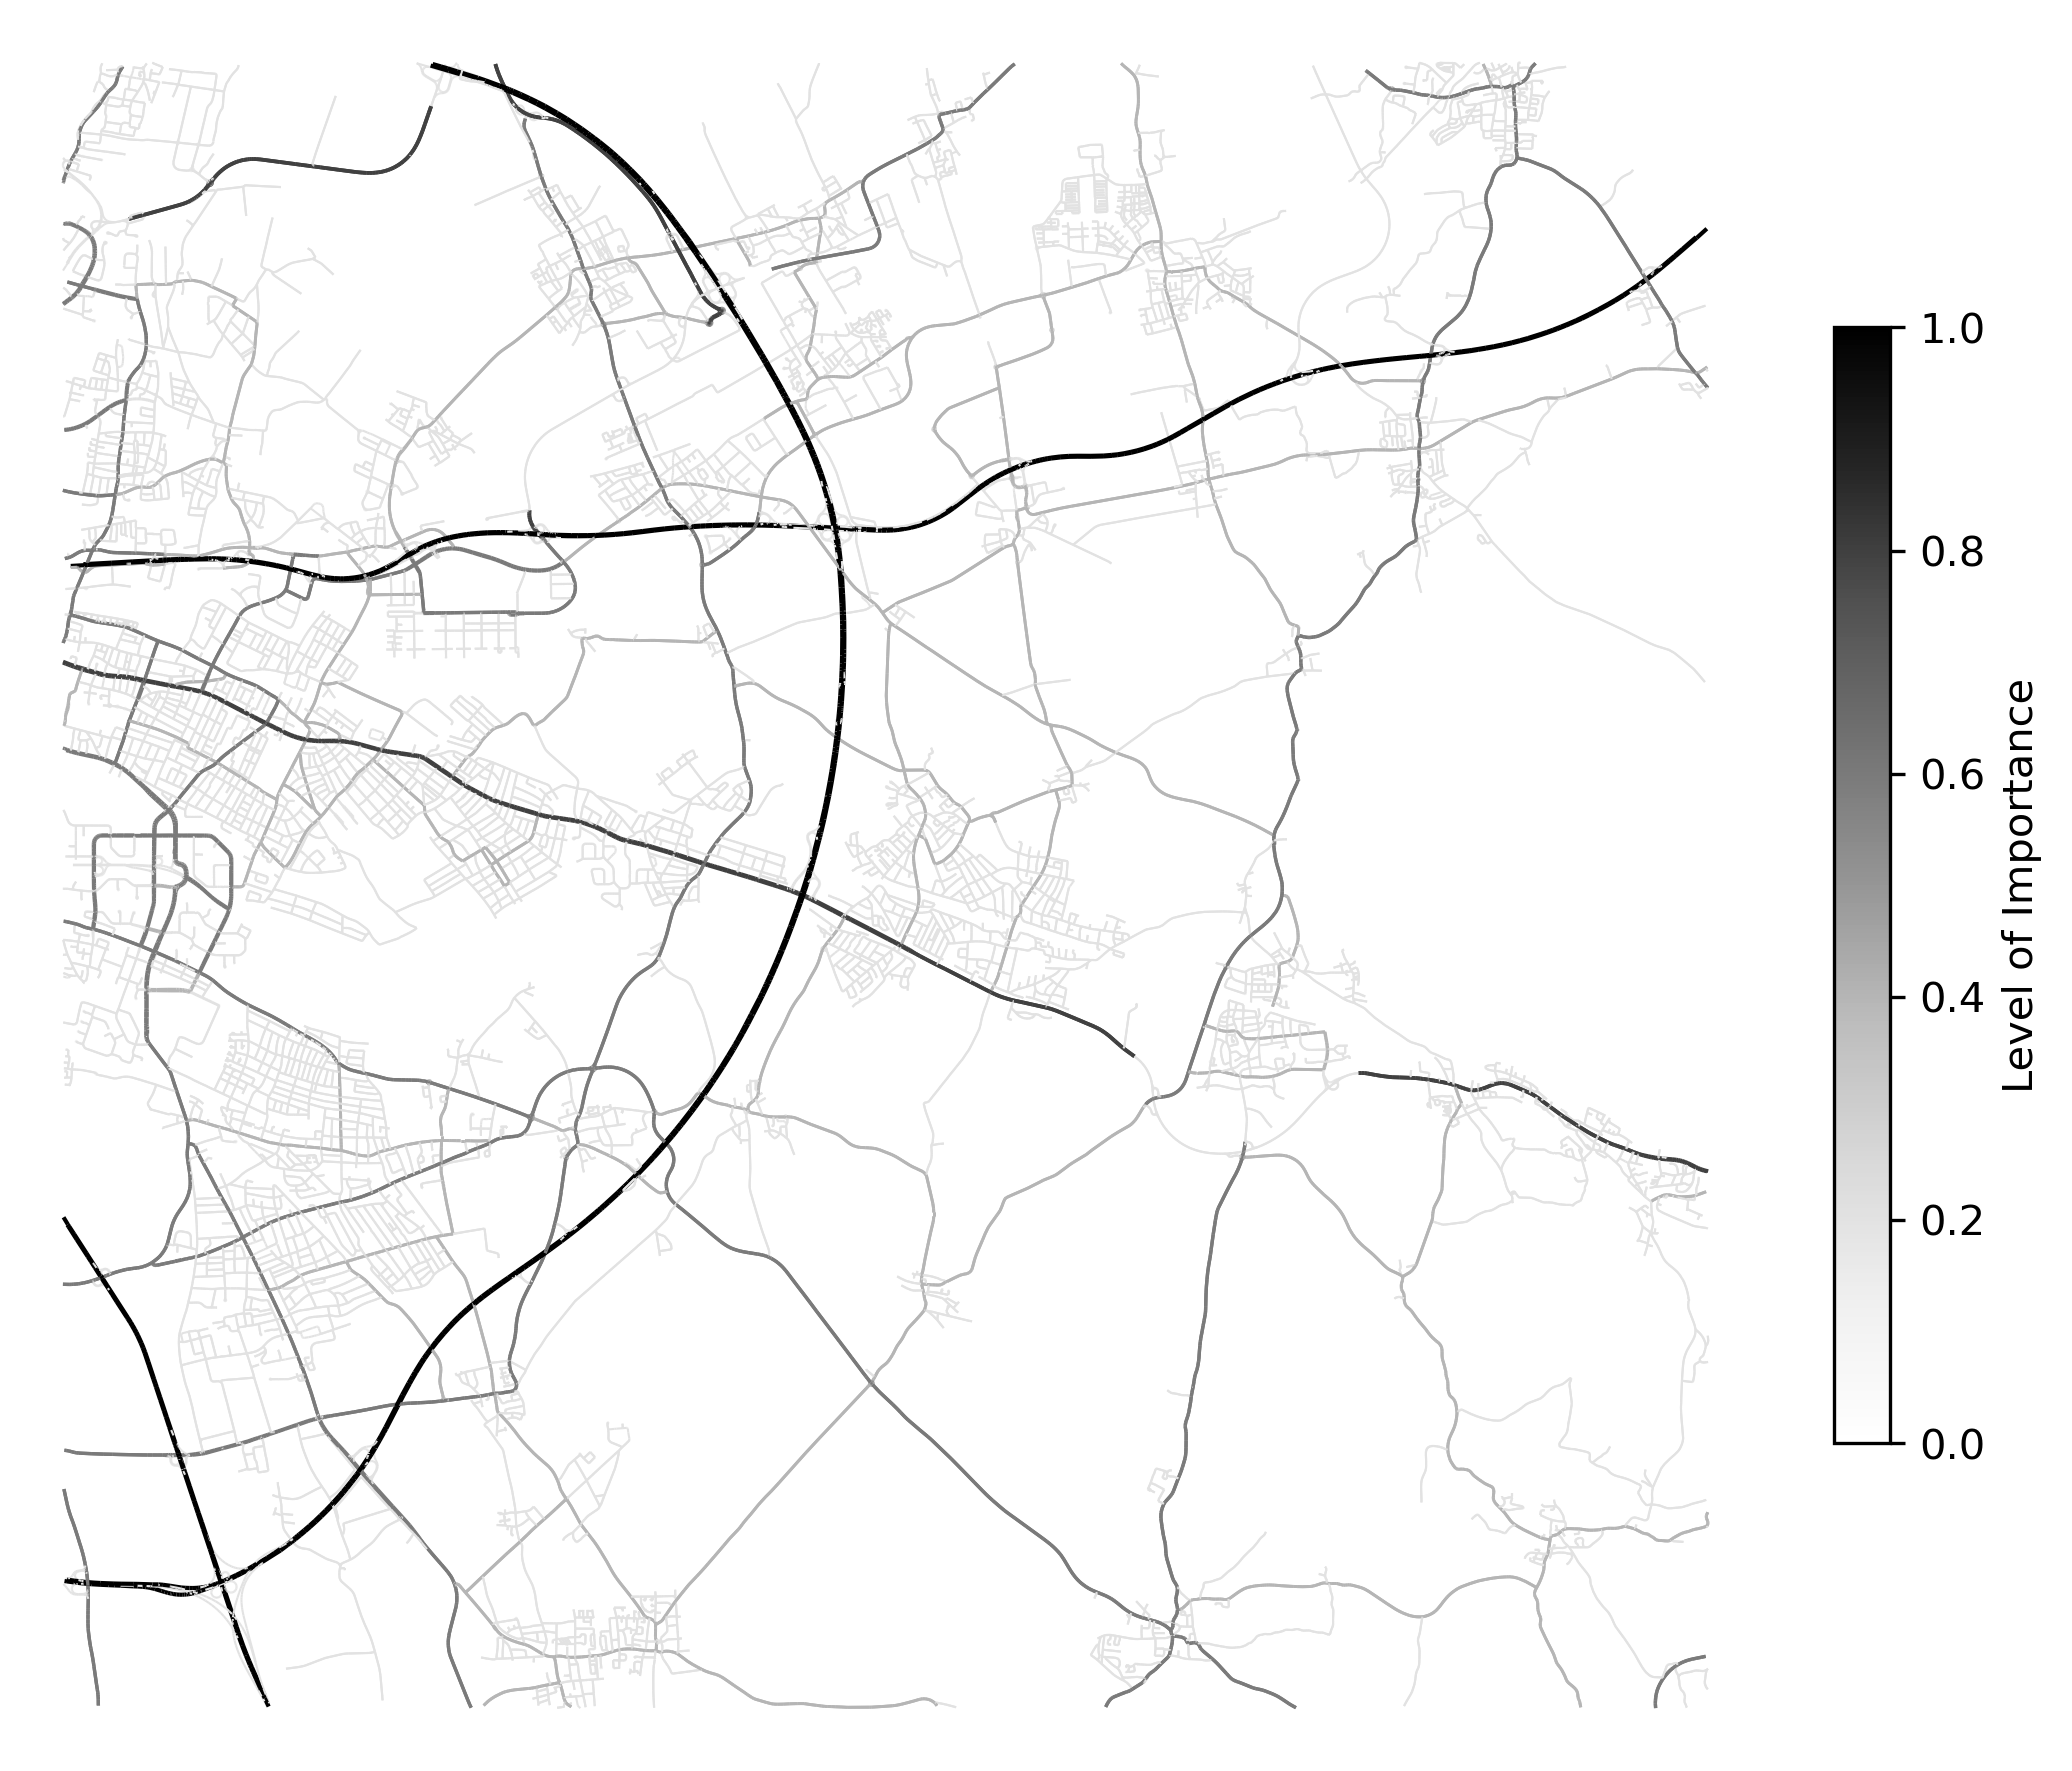
\includegraphics[width=0.5\textwidth]{figures/road_hierarchy.png}
    \caption[Hierarchie in Straßennetzen]{Hierarchie in Straßennetzen. Autobahnen (schwarz) sind
        ganz oben in der Hierarchie und sind sehr "`wichtig"'. Dagegen sind Straßen in
        Wohnsiedlungen weniger wichtig. \osmcr}
    \label{fig:road_hierarchy}
\end{figure}
Die Methode der Contraction Hierarchies nach Geisberger et al.
\cite{geisberger.workshop}~\cite{geisberger.thesis}~\cite{geisberger.exact} löst dieses Problem,
indem in einer Vorverarbeitungsphase Abkürzungskanten in den Graph eingefügt werden, die in der
Suche ausgenutzt werden. Die Abkürzungen erhalten dabei die kürzesten Wege \cite{Bast.20.04.2015}.
Während der Suche wird ein modifizieren bidirektioanlen Dijkstra-Algorithmus angewendet, der Kanten
die zu Knoten mit niedrigerem Level führen ignoriert. Dadurch wird der Suchraum extrem verkleinert,
was zu schnellen Antwortzeiten führt. Der CH-Algorithmus lässt sich in zwei Komponenten unterteilen:
\begin{enumerate}
    \item Vorverarbeitung: In dieser Phase werden die Knoten geordnet und die Hierarchie augebaut.
    \item Suche: Ausführung der bidirektionale Suche auf dem erweiterten Graph.
\end{enumerate}


\subsubsection{Vorverarbeitung}
In dieser Phase wird der Graph $G = (V,E)$ um zusätzliche Abkürzungskanten erweitert. Die
Abkürzungskanten werden im Prozess der Knotenkontraktion (eng. Node Contraction) eingefügt. Wenn ein
Knoten $v \in V$ \emph{kontraktiert} wird, dann wird er und alle Kanten die mit $v$ inzident sind
aus dem Graphen entfernt. Der Zeitpunkt des Entfernens ist gleichzeitig das \emph{Level} des
Knotens. Je später der Knoten entfernt wird, desto höher ist sein Level und damit seine Relevanz.
Wenn $v$ auf dem kürzesten Weg zwischen zwei benachbarten Knoten $u$ und $w$ liegt, dann wird eine
Abkürzungskante $e(u,w)$ mit $w(u,w) = w(u,v) + w(v,w)$ eingefügt, um den kürzesten Weg zu erhalten.

Abbildung~\ref{fig:ex_contraction} demonstriert den Prozess: Knoten $v$ soll kontraktiert werden und
damit er und seine inzidenten Kanten entfernt werden. Sei $U$ die Menge aller eingehenden Kanten und
$W$ die Menge aller ausgehenden Kanten, dann muss für jedes Paar überprüft werden, ob $v$ auf dem
kürzesten Weg <$u,v,w$> zwischen zwei benachbarten Knoten $u \in U$ mit $Level(u) > Level(v)$ und $w
    \in W$ mit $Level(w) > Level(v)$ liegt. Zum Beispiel ist dies zwischen $u_1$ und $w_2$ der Fall,
denn es gibt keine andere Möglichkeit $w_2$ zu erreichen, als über $v$. Um den kürzesten Weg zu
erhalten, wird eine Abkürzungskante $e(u_1,w_2)$ mit dem Gewicht
$w(u_1,w_2)=w(u_1,v)+w(v,w_2)=1+1=2$ eingefügt. Das gleiche gilt für <$u_2,v,w_1$> und
<$u_2,v,w_2$>. Der Weg von $u_1$ nach $w_1$ kann allerding über <$u_1,x,y,w_1$> schneller erreicht
werden (Kosten 3 sind kleiner als 4) und es muss daher keine Abkürzungskante eingefügt werden.
\begin{figure}[h]
    \centering
    \begin{subfigure}[b]{0.45\textwidth}
        \centering
        \begin{tikzpicture}
            \Vertex[x=0,y=0,label=v]{v}
            \Vertex[x=-2.5,y=1.5,label=$u_1$]{u1}
            \Vertex[x=-2.5,y=-1.5,label=$u_2$]{u2}
            \Vertex[x=-1,y=2,label=x]{x}
            \Vertex[x=1,y=2,label=y]{y}
            \Vertex[x=2.5,y=1.5,label=$w_1$]{w1}
            \Vertex[x=2.5,y=-1.5,label=$w_2$]{w2}
            \Edge[label=1](u1)(v)
            \Edge[label=1](u2)(v)
            \Edge[label=3](v)(w1)
            \Edge[label=1](v)(w2)
            \Edge[label=1](u1)(x)
            \Edge[label=1](x)(y)
            \Edge[label=1](y)(w1)
        \end{tikzpicture}
        \caption{Graph $G = (V,E)$}
    \end{subfigure}
    \begin{subfigure}[b]{0.45\textwidth}
        \centering
        \begin{tikzpicture}
            \SetVertexStyle[TextOpacity=0.2,FillColor=white,LineOpacity=0.2]
            \Vertex[x=0,y=0,label=v,opacity=0.2]{v}
            \SetVertexStyle[TextOpacity=1,FillColor=white,LineOpacity=1]
            \Vertex[x=-2.5,y=1.5,label=$u_1$]{u1}
            \Vertex[x=-2.5,y=-1.5,label=$u_2$]{u2}
            \Vertex[x=-1,y=2,label=x]{x}
            \Vertex[x=1,y=2,label=y]{y}
            \Vertex[x=2.5,y=1.5,label=$w_1$]{w1}
            \Vertex[x=2.5,y=-1.5,label=$w_2$]{w2}
            \SetEdgeStyle[TextOpacity=0.2,TextFillOpacity=0.2,Opacity=0.2]
            \Edge[label=1](u1)(v)
            \Edge[label=1](u2)(v)
            \Edge[label=3](v)(w1)
            \Edge[label=1](v)(w2)
            \SetEdgeStyle[TextOpacity=1,TextFillOpacity=1,Opacity=1]
            \Edge[label=1](u1)(x)
            \Edge[label=1](x)(y)
            \Edge[label=1](y)(w1)
            \Edge[fontsize=\large,label=2,color=red,bend=10,Direct,style=dashed,distance=0.3](u1)(w2)
            \Edge[fontsize=\large,label=4,color=red,bend=10,Direct,style=dashed,distance=0.3](u2)(w1)
            \Edge[fontsize=\large,label=2,color=red,bend=10,Direct,style=dashed](u2)(w2)
        \end{tikzpicture}
        \caption{Graph $G' = (V', E')$ mit $V' = V - \{v\}$}
    \end{subfigure}
    \caption[Knotenkontraktion]{Beispiel einer Knotenkontraktion}
    \label{fig:ex_contraction}
\end{figure}

Nachdem jeder Knoten kontraktiert wurde, erhält man einen neuen Graph  ${G^{*} = (V,E')}$, der als
\emph{Overlaygraphh} bezeichnet wird. $E'$ enthält alle ursprünglichen Kanten sowie die neu
hinzugefügten Abkürzungskanten (siehe Abbildung~\ref{fig:overlaygraph}).

Algorithmus zur Erstellung einer \ac{CH}

\begin{algorithm}[H]
    \caption{RUN\_CONTRACTION(G)}
    \label{algo:contraction}
    \begin{algorithmic}
        \ForEach{$v \in V$ geordnet nach Level}
        \ForEach{$(u,v) \in E$ mit $Level(u) > Level(v)$}
        \ForEach{$(v,w) \in E$ mit $Level(w) > Level(v)$}
        \If{<u,v,w> ist kürzester Weg von $u$ nach $w$}
        \State $E = E \cup \{e(u,w)\}$ mit Gewicht ${w(u,w) = w(u,v) + w(v,w)}$
        \EndIf
        \EndFor
        \EndFor
        \EndFor
    \end{algorithmic}
\end{algorithm}

\textbf{Beweis: Kontraktion erhält kürzeste Wege}
\begin{lemma}
    Sei $G = (V,E)$ ein beliebiger Graph und $G' = (V',E')$ der Graph nach Kontratkion von einem
    beliebigen Knoten $v \in V$ mit $V' = V - \{v\}$.\\
    Dann gilt für alle $s,t \in V'$: ${dist_{G'}(s,t) = dist_{G}(s,t)}$.
\end{lemma}
Lorem ipsum dolor sit amet, consectetur adipiscing elit. Sed euismod, nisl quis tincidunt
pellentesque, nunc nisl ultrices ipsum, quis aliquam nunc nisl ut nunc. Nulla facilisi. Nulla


\SetVertexStyle[MinSize = 4.5mm]
\SetLayerDistance{-7}
\SetPlaneWidth{15}
\SetPlaneHeight{7}
\begin{figure}
    \centering
    \begin{tikzpicture}[multilayer=3d,xscale=.5,yscale=.5]
        %
        % Layer 2

        % Background
        \Plane[layer=2,x=1,y=1,NoBorder,InBG]

        % Text
        \Text[x=1.2,y=0.8,layer=2,anchor=north west,style={scale=2.0}]{Originalgraph $G$}

        % Vertices
        \Vertices[color=orange]{data/graphs/ex3/vertices.csv}

        % Intra-layer edges in layer 2
        \Edges[layer={2,2},NoLabel]{data/graphs/ex3/edges_with_shortcuts.csv}
        \EdgesNotInBG

        % Inter-layer edges between layer 1 and 2
        \Edges[color=black,NoLabel,layer={1,2},style={dashed}]{data/graphs/ex3/edges_with_shortcuts.csv}

        %%
        % Layer 1

        % Background
        \Plane[x=1,y=1,NoBorder,color=orange]

        % Text
        \Text[x=1.2,y=0.8,layer=1,anchor=north west,style={scale=2.0}]{Overlaygraph $G^{*}$}

        % Intra-layer edges in layer 1
        \Edges[layer={1,1},NoLabel]{data/graphs/ex3/edges_with_shortcuts.csv}

        % Vertices in layer 1
        \Vertices[layer=1,color=blue]{data/graphs/ex3/vertices.csv}


    \end{tikzpicture}
    \caption[Overlaygraph]{Overlaygraph nach Kontraktionsprozess. Der Graph $G^{*}$ enthält alle
        ursprünglichen Kanten sowie die neu hinzugefügten Abkürzungskanten.}
    \label{fig:overlaygraph}
\end{figure}

\subsubsection{Suche}